
%(BEGIN_QUESTION)
% Copyright 2013, Tony R. Kuphaldt, released under the Creative Commons Attribution License (v 1.0)
% This means you may do almost anything with this work of mine, so long as you give me proper credit

Calculate the temperature of the process if the voltmeter registers 21.699 mV when connected to the terminals in the thermocouple head:

$$\includegraphics[width=15.5cm]{i02900x01.eps}$$

$T_{process}$ = \underbar{\hskip 50pt} degrees F

\underbar{file i02900}
%(END_QUESTION)





%(BEGIN_ANSWER)

$T_{process}$ = \underbar{\bf 1034} degrees F
 
%(END_ANSWER)





%(BEGIN_NOTES)

{\bf This question is intended for exams only and not worksheets!}.

%(END_NOTES)


